% define coloring in language JavaScript
\definecolor{lightgray}{rgb}{.9,.9,.9}
\definecolor{darkgray}{rgb}{.4,.4,.4}
\definecolor{purple}{rgb}{0.65, 0.12, 0.82}
\lstdefinelanguage{JavaScript}{
  keywords={break, case, catch, continue, debugger, default, delete, do, else, false, finally, for, function, if, in, instanceof, new, null, return, switch, this, throw, true, try, typeof, var, void, while, with},
  morecomment=[l]{//},
  morecomment=[s]{/*}{*/},
  morestring=[b]',
  morestring=[b]",
  ndkeywords={class, export, boolean, throw, implements, import, this},
  keywordstyle=\color{blue}\bfseries,
  ndkeywordstyle=\color{darkgray}\bfseries,
  identifierstyle=\color{black},
  commentstyle=\color{purple}\ttfamily,
  stringstyle=\color{red}\ttfamily,
  sensitive=true
}

\section{Cieľ práce}
Všeobecným cieľom diplomovej práce je analyzovať existujúce riešenia virtuálnych laboratoratórií a možností Node.js pre vytvorenie nového.
Na základe zistených možností je potrebné vytvoriť virtuálne laboratórium ako klient-server architektúru, kde server bude Node.js a klienti matlab a webová aplikácia v prehliadači. Experiment vrámci virtualného laboratória prebieha ako simulácia v Matlabe cez rozšírenie Simulink. Táto aplikácia nebude obmedzená len na lokálnu sieť, ale bude prístupna aj z internetu. Klient aj server bude vytvorený v dynamicky typovanom jazyku JavaScript. Údaje z experimentu sa budú zasielať z Matlabu na server cez websockety, kde môžu byť následne spracované a uložené do databázy, alebo zaslané klientovi do prehliadača.


\section{Virtuálne laboratória}
\indent V dobe keď internet ešte nebol rozšírený, experimenty sa robili vo fyzických laboratóriach. Bolo potrebné dodržiavať isté bezpečnostné predpisy, kvôli možnému úrazu osoby alebo možnému poškodeniu nástrojov.\\
\indent Vzdialenosť a hlavne nedostatok finančných zdrojov nám sťažuje podmienky pri testovaní experimentov, hlavne v prípadoch ked je potrebné mať pokrokové sofistikované nástroje. Ďalší problém s ktorým sa stretávame je nedostatok kvalitných lektorov. V dnešnej dobe existujú online kurzy, ktoré poskytujú aj video ukážky, ale to tento problém rieši len čiastočne. Vždy bolo výzvou vykonávanie spoločných experimentov viacerými inštitúciami súčasne a zároveň zdielanie nákladov na prostriedky. V súčasnej dobe internetu a počítačových technológií už tieto obmedzenia nemusia trápiť študentov ani výskumníkov. Internet umožnil to, že experimenty môžu byť štruktorované tak, aby boli ovládané a prezerané na ďiaľku. Práve to by pomohlo v učení v základných ale aj pokročilých konceptov prostredníctvom vzdialeného experimentovania. V súčasnosti veľa vybavenia už poskytuje rozhranie pre pripojenie počítača a spracovanie dát z neho. Vďaka tomu je možné navrhnúť experimenty, ktoré pomôžu študentom pri učení. Experimentovanie cez internet umožňuje využívanie zdrojov, znalostí, software a dát z  internetu narozdiel od fyzických experimentov, ktoré by vznikali súčasne na rôznych miestach.\cite{vlabphylosopfy}\\
\indent V tejto práci sa budeme zaoberať tvorbou virtuálneho laboratória (ďalej len VL). Predtým ako si popíšeme detailné fungovanie technológií pre vytvorenie VL, si musíme vysvetliť čo považujeme za VL, pochopiť aké hodnoty nám môže priniesť, ale samozrejme aj tie ktoré nemôže. Vo všeobecnosti môžme povedať ze VL je počítačový program, kde študenti sú v interakcii s experimentom prostredníctvom počítača. Typický príklad je simulácia experimentu, kedy je študent v interakcii s naprogramovaným rozhraním. Ďalšia možnosť je diaľkovo ovládaný experiment, kde študent je v interakcii s reálnym zariadením cez počítačové rozhranie, napriek tomu že sa nenachádza pri ňom. Keď vylúčime druhú variantu tak si môžme utvoriť definíciu nasledovne: \textit{Virtuálnym laboratóriom voláme to, keď je študent študent v interakcií s experimentom, ktorá je od neho fyzicky vzdialená alebo nemá za sebou žiadnu fyzickú realitu.}\cite{hatherly}

\begin{figure}[H]
  \centering
  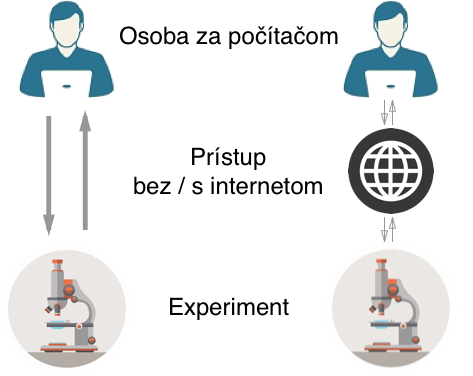
\includegraphics[scale=0.5]{img/VL_vs_real.png}
  \caption{Porovnanie medzi počítačovo riadneným experimentom vľavo a vzdialene riadeným experimentom vpravo.}
  \label{img-real-vs-vl}
\end{figure}

Po vysvetlení čo je VL sa pozrieme na výhody, ktoré nám môže priniesť. Sú popísané v bodoch v \textit{tabuľke č.\ref{table-real-remote-virtual-laboratory}.}
Človek často radí medzi "výhody" to, že môže nahradiť fyzické laboratória. Lenže to medzi výhody nepatrí. Nie je možné nahradiť skúsenosti z fyzickej práce zo zariadením VL aj keď je to lepšie ako žiadna skúsenosť. VL by nemalo byť vnímané tak, že poskytuje maximálnu možnú skúsenosť.
\begin{table}[H]
\small
\begin{tabular}{l l l}
\hline
\textbf{Typ laboratória} & \textbf{Výhody}  & \textbf{Nevýhody} \\ \hline
\textbf{Fyzické} & realistické dáta & obmedzenia na čase a mieste \\
& interakcia s reálnym zariadením & potrebné plánovanie prístupu\\
& lepšia spolupráca & nákladnosť experimentu \\
& interakcia s lektorom & potrebný lektor \\ \hline
\textbf{Virtuálne} & dobré pre vysvetlenie konceptu &  idealizované dáta\\
& bez obmedzenia na čas a miesto &  nedostatok spolupráce  \\
& interaktívne médium & bez interakcie s reálnym zariadením \\
& nízke náklady & \\ \hline
\textbf{Vzdialené} & interakcia s reálnym zariadením &  "virtuálna" prítomnosť v laboratóriu \\
& kalibrácia & \\
& realistické dáta & \\
& bez obmedzenia na čas a miesto & \\
& stredné náklady & \\ \hline
\end{tabular}
\caption{Porovnanie fyzických, virtuálnych a vzdialených a laboratórií}
\label{table-real-remote-virtual-laboratory}
\end{table}

\subsection{Prehľad existujúcich virtuálnych laboratórií}
V dobe písania tohto dokumentu existuje množstvo rôznych virtuálnych/vzdialených laboratórií, ktoré používajú zahraničné školy pre výučbu alebo výskum. V práci \cite{vlabtablecomparison} je zoznam veľmi používaných laboratórií, ktoré sú prístupne cez internet. Porovnanie funkcionality a využitých technológií je možné vidieť v  \textit{tabuľke č.\ref{table-vlab-comparison}.}

\begin{table}[H]
\scriptsize
\begin{tabular}{l l l l}
\hline\hline
\textbf{Názov} & \textbf{Klient} & \textbf{Server} & \textbf{Prevedenie}\\ \hline
Weblab-DEUSTO & AJAX, Flash, Java applets, & Web services, Python, LabVIEW, & Xilinx-VHDL, LabView\\
&LabVIEW, Remote panel & Java, .NET, C, C++ &\\ \hline
NCSLab & AJAX, Flash & PHP & Matlab, Simulink\\ \hline
ACT & HTML, Java Applets & PHP & Matlab, Simulink\\ \hline
LabShare Sahara & AJAX, Java applets & Web services, Java & Java\\ \hline
iLab & HTML, ActiveX, Java applets & Web services, .NET & LabVIEW\\ \hline
RECOLAB & HTML & PHP & Matlab, Simulink\\ \hline
SLD & AJAX, HTML & Web services, PHP & Matlab, Simulink\\ \hline\hline
\end{tabular}
\caption{Porovnanie virtuálnych laboratórií vytvorených mimo FEI STU.}
\label{table-vlab-comparison}
\end{table}

Následne som preskúmal možnosti existujúcich riešení v \textit{tabuľke č.\ref{table-feistu}}, ktoré boli vytvorené na Fakulte elektrotechniky a informatiky STU.\cite{table-vlab-farkas}\cite{table-vlab-borka}\cite{table-vlab-kundrat}\cite{table-vlab-cerveny}\cite{table-vlab-varga}
\begin{table}[H]
\tiny
\begin{tabular}{l l l l l l}
\hline\hline
\textbf{Rok vypracovania}  & \textbf{Autor} & \textbf{Prevedenie} & \textbf{Spôsob komunikácie} & \textbf{Klient} & \textbf{Server}\\ \hline
2011 &  Roman FARKAŠ & Matlab & JMI, sockets & Java & Java\\
&& Simulink &&& \\
&& Reálna sústava &&& \\ \hline
2012 &  Tibor BORKA  & Matlab & WCF & .NET, WPF & .NET\\
&& Simulink &&& \\
&& Reálna sústava &&& \\ \hline
2014 &  Michal KUNDRÁT  & Matlab & JMI, SOAP & HTML, JS & Tomcat, Java, \\
&& Simulink &&& JSF, EJB3\\ 
&&&&& MySQL\\ \hline
2014 &  Tomáš ČERVENÝ  & Matlab & JMI, HTTP & Mobilné HTML, JS & Jetty, Java\\
&& Simulink &&& \\ \hline
2015 &  Štefan VARGA  & Matlab & COM, HTTP & HTML, JS & PHP, .NET\\
&& Simulink &&& \\ \hline\hline
\end{tabular}
\caption{Porovnanie virtuálnych laboratórií vytvorených na FEI STU.}
\label{table-feistu}
\end{table}

\subsubsection{Nevýhody existujúcich riešení}
Pri tvorbe softwarového systému, či už všeobecne, alebo v našom prípade virtuálneho laboratória je vhodné preskúmať možnosti existujúcich riešení. Robí sa to kvôli tomu, aby sme sa pri návrhu vyvarovali rôznym chybám ktoré môžu nastať, alebo technológiam, ktoré už časom zastarali. V dnešnej dobe je vývoj nových technológií neskutočne rýchly. Takúto analýzu existujúch riešení sme spravili v predchádzajúcej sekcii.
Naša téma je zameraná na vytvorenie multiplatformového riešenia, kde nie je možné využiť WCF ani COM technológie ako v predchádzajúcich riešeniach. JMI je zase vhodné len pre riešenie, kde sa využíva Java. Pre server nie je možné využiť technológie LabVIEW, .NET (momentálne je vo vývoji multiplatformová verzia). Čo sa týka klienských riešení tak Flash, ActiveX, Java applets už nie sú podporované v prehliadačoch, taktiež ich nie je vhodné použiť.

\subsection{Komponenty virtuálneho laboratória}
Počet existujúcich laboratórií je veľký, ale väčšinou nie je možné zaručiť kompatibilitu, pretože tu neexistuje žiadny štandard. Ale vždy je možné identifikovať základné komponenty, ktoré tieto VL využívajú. Niektoré z nich môžu byť dokonca využité viac krát.\cite{article-components-vl}

\begin{enumerate}
  \item Samotný experiment
  \item Zariadenie umožnujúce kontrolu experimentu a získavanie hodnôt z neho.
  \item Laboratórny server, ktorý zabezpečí kontrolu, monitorovanie a spracovanie dát z experimentu.
  \item Server, ktorý zabezpečí prepojenie medzi vzdialenými uživateľmi a laboratórneho servera, zvyčajne prostredníctvom internetu.
  \item Webová kamera pripojená k serveru, ktorá môže byť použitá pre vzdialeného používateľa ako vizuálna a zvuková spätná väzba o stave experimentu.
  \item Nástroje umožňujúce viacužívateľské audio, video a chat komunikáciu.
  \item Klientské zariadenia, ktoré sa pripoja vzdialene k experimentu. Väčšinou sa jedná o webovú aplikáciu alebo java aplikáciu.
\end{enumerate}

Je ale dôležité si uvedomiť, že na vytvorenie laboratória nepotrebujeme všetky tieto komponenty, resp. môžme využiť aj iné, ktoré sa nám dokonale hodia. Niekedy sa používa napr. aj databázový server ak chceme experimenty ukladať a spracovávať neskôr. Tak isto je potrebné uvedomiť si, aký typ VL chceme vytvoriť. Určite budú rozdiely pri návrhu jednoužívateľského VL narozdiel od viacužívateľského dokonca s viacerými experimentami súčasne. Treba myslieť na to, ako vhodne vyriešiť škálovateľnosť, možné problémy s bezpečnosťou, viacužívateľský prístup, ostatné problémy prístupnosti a podobne.


\section{Použíté technológie}\label{used-technologies}
V predchádzajúcich kapitolách sme popísali cieľe, čo chceme vlastne dosiahnuť. Ďalej sme analyzovali možnosti virtuálnych laboratórií a porovnali už s existujúcimi riešeniami. V tejto sekcii budú v krátkosti rozpísané použité technológie. Je samozrejmé, že nie je možné ku každej popísať všetky jej možnosti, ale budeme sa venovať hlavne tým, ktoré plánujeme využiť aj v implementácií.

\subsection{Matlab R2015b}
Milióny inžinierov a vedcov na celom svete používajú MATLAB na analýzu a návrh systémov a produktov ktore menia náš svet. MATLAB sa používa v automobilových systémoch, vesmírnych staniciach, smart siete, mobilých sieťach LTE alebo aj v škole na štúdium. Ďalej sa používa pre strojové učenie, spracovanie signálu, spracovanie obrazu, počítačové videnie, komunikácie, finančníctvo, riadenie, robotika a mnoho ďalšich využití.
Celá platforma MATLAB je optimalizovaná pre riešenie inžinierskych a vedeckých problémov. Jazyk MATLABu je založený na práci s maticami. Je považovaný za najprirodzenejší spôsob ako počítať matematické úlohy. Pomocou integrovanej grafickej knižnici je možné vizualizovať a získať výsledky z dát. MATLAB integruje aj množstvo toolboxov, ktoré pomáhajú priamo začať s algoritmami, ktoré potrebujeme pre našu doménu.\cite{matlab-mathworks}

\subsubsection{Simulink}
Matlab obsahuje viacero integrovaných nástrojov a jeden z nich je aj Simulink. Je to grafické rozhranie, v ktorom je možné modelovať, simulovať a potom aj analyzovať dynamické systémy. Jeho hlavné rozhranie je grafické plátno, kde možme spájať jednotlivé bloky do diagramu. Simulink vie úzko spolupracovať s matlabom, dokonca môže byť odtiaľ aj skriptovaný, resp. počiatočná inicializácia hodnôt. Matlab a simulink sú vlastne dve prostredia integrované do jedného software. Čiže je možné simulovať a analyzovať náš model v každom kroku simulácie v oboch prostrediach. Simulink väčšinou spúštame priamo z Matlabu.

\subsubsection{Komunikácia medzi Matlabom a Node.js}
Simulácia dynamickej sústavy, ktorá sa spustí v Simulinku môže odosielať výsledné dáta do Matlab workspace. Odtiaľ ich budeme chciet posielať do Node.js na ďalšie spracovanie. V matlabe existuje viacero možností získania dát z workspace.\\\\
\textbf{COM} (Component Object Model) je prvá z technologických možností. COM bolo vytvorené spoločnosťou Microsoft, čiže toto riešenie je obmedzené len na Windows platformu. Používajú sa na prepojenie rôznych aplikácií podporujúcich túto technológiu. Tieto objekty môžu byť vytvorené pomocou rôznych programovacích jazykov ako napr. C++ alebo Java.\cite{matlab-microsoft-com}\\
Kým idea COM je celkom jasná, terminológia až toľko nie. \textit{COM object} je softwarový komponent, ktorá zodpovedá Component Object Model. COM vnucuje zapuzdrenie objektu a tým predchádza pred priamym prístupom do dát a implementácie. COM objekt poskytne rozhranie, ktoré obsahuje premenné, metódy a udalosti. \textit{COM client} je program, ktorý používa COM objekty. COM objekty, ktorý poskytujú funkcionalitu pre použitie sú volané COM server. COM server môže byť in-process alebo out-of-process. Príklad out-of-process servera je napríklad Microsoft Excel. \textit{Microsoft ActiveX control} je typ in-process COM servera, ktorý vyžaduje kontainer. ActiveX zvyčajne poskytuje užívateľské rozhranie. Príkladom môže byť Microsoft Calendar control. Control container je aplikácia schopná poskytovať ActiveX prvky. Matlab figure okno alebo Simulink model su tiež príklady control kontajnerov. Matlab može byť použitý aj ako COM klient aj ako COM automation server.\cite{matlab-com}\\

\textbf{Websockety}
popisat matlab webscokety -- narocnejsie implementovat, pretoze nie je nativna implementacia\\
%
% Dlhy komentaaaaaaaaaaaaaaaaaaaaaaaaaaaaaar
% 

\textbf{RESTful web service}
Medzi najmodernejšie možnosti komunikácie Matlabu s vonkajškom patria jednoznačne RESTful služby. REST (representational state transfer) je softwarový architektonický štýl, pomocou ktorého vieme posielať a získavať dáta zo serveru. REST komunikuje pomocou HTTP/HTTPS protokolu a zväčša sa používa na CRUD aplikácie, čiže tam kde chceme robiť CREATE, READ, UPDATE, DELETE operácie. Dáta je možné vymieňať medzi klientom a serverom cez \textit{JSON} alebo \textit{XML} správ. Pre jednoduchšie projekty sa používajú skôr JSON, hlavne ak sa maju spracovávať JavaScriptom. Výhodou RESTful v tomto riešení je to, že je priamo implementované v Matlabe a nie je potrebné inštalovať ďalšie knižnice a toolboxy.

\begin{figure}[H]
  \centering
  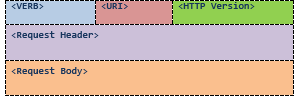
\includegraphics[scale=0.7]{img/rest/rest-http.png}
  \caption{HTTP request.}
  \label{rest-http}
\end{figure}

Na obrázku č.\ref{rest-http} vidíme ako vyzerá HTTP request. V položke \textit{<VERB>} sa nachádza jedna z HTTP metód GET, PUT, POST, DELETE, OPTIONS, ... V \textit{<URI>} je zase linka na zdroj, nad ktorým sa bude vykonávať daná operácia. \textit{<HTTP version>} je verzia HTTP, vo všeobecnosti to bude "HTTP v1.1" ale môže byť aj "HTTP v2.0" v novších systémoch.\\
\textit{<Request Header>} obsahuje metadáta ako kolekciu párov "key" : "value" hlavičky. Tieto nastavenia obsahujú informáciu o správe a jej odosielateľovi ako typ klienta, aký formát podporuje klient, typ formátu správy tela, nastavenia cache pre odpoveď a mnohé ďalšie informácie.\\
\textit{<Request Body>} je aktuálny obsah správy. V RESTful službách je toto miesta, kde sa nachádza obsah správy, ktorý sa vymieňa medzi klientom a serverom. V tejto časti nie sú žiadne tagy ani značky pre učenie začiatku alebo konca správy.\cite{rest-vaqqas}

\begin{algorithm}[H]
\lstset{
   language=XML,
   backgroundcolor=\color{lightgray},
   extendedchars=true,
   basicstyle=\footnotesize\ttfamily,
   showstringspaces=false,
   showspaces=false,
   numbers=none,
   numberstyle=\footnotesize,
   numbersep=9pt,
   tabsize=2,
   breaklines=true,
   showtabs=false,
   captionpos=b
}
\begin{lstlisting}
POST http://MyService/Person/
Host: MyService
Content-Type: text/xml; charset=utf-8
Content-Length: 123
<?xml version="1.0" encoding="utf-8"?>
<Person>
  <ID>1</ID>
  <Name>M Vaqqas</Name>
  <Email>m.vaqqas@gmail.com</Email>
  <Country>India</Country>
</Person>
\end{lstlisting}
 \caption{Príklad POST requestu.}
 \label{post-request}
\end{algorithm}

\begin{algorithm}[H]
\lstset{
   language=XML,
   backgroundcolor=\color{lightgray},
   extendedchars=true,
   basicstyle=\footnotesize\ttfamily,
   showstringspaces=false,
   showspaces=false,
   numbers=none,
   numberstyle=\footnotesize,
   numbersep=9pt,
   tabsize=2,
   breaklines=true,
   showtabs=false,
   captionpos=b
}
\begin{lstlisting}
HTTP/1.1 200 OK
Date: Sat, 23 Aug 2014 18:31:04 GMT
Server: Apache/2
Last-Modified: Wed, 01 Sep 2004 13:24:52 GMT
Accept-Ranges: bytes
Content-Length: 32859
Cache-Control: max-age=21600, must-revalidate
Expires: Sun, 24 Aug 2014 00:31:04 GMT
Content-Type: text/html; charset=iso-8859-1
<!DOCTYPE html PUBLIC "-//W3C//DTD XHTML 1.0 Strict//EN" "http://www.w3.org/TR/xhtml1/DTD/xhtml1-strict.dtd">
<html xmlns='http://www.w3.org/1999/xhtml'>
<head><title>Hypertext Transfer Protocol -- HTTP/1.1</title></head>
<body>
...
\end{lstlisting}
 \caption{Príklad GET requestu.}
 \label{get-request}
\end{algorithm}

V ukážke POST requestu č.\ref{post-request} zasielame serveru XML s údajmi o novej osobe. V ukážke GET requestu č.\ref{get-request} je vidieť, že server vráti obsah HTML stránky na ktorú bola požiadavka vytvorená.

Teraz keď sme si vysvetlili v stručnosti ako fungujú RESTful služby, tak sa dostávame k tomu ako ich je možné využiť z Matlabu. Matlab poskytuje viacero funkcií na prácu s REST ako \textit{weboptions}, \textit{webread}, \textit{webwrite}.\\
Objekt \textit{weboptions} slúži na špecifikáciu parametrov pre RESTful službu. V Matlabe sa volá príkazom \textit{options = weboptions} alebo \textit{options = weboptions(Name,Value)} pričom \textit{Name} je názov parametra, ktorý chceme nastaviť a \textit{Value} jeho hodnota.\\
Je možné nastaviť tieto parametre: \textit{CharacterEncoding, UserAgent, Timeout, Username, Password, KeyName, KeyValue, ContentType, ContentReader, MediaType, RequestMethod, ArrayFormat}. Ak chceme zobraziť objekt weboptions, tak namiesto hesla tam budú hviezdičky. Každopádne, objekt ukladá heslo ako čistý text. V prípade keď zavoláme túto vlastnosť v Matlabe cez options.Password tak heslo bude viditeľné.\ref{matlab-weboptions}\\
Objekt \textit{webread} číta obsah z REST služby, na ktorú sme mu poskytli URL cestu a vráti obsah ako štruktúru do požadovanej premennej. Existujú tri najpoužívanejšie možnosti použitia. \textit{data = webread(url)} kde parameter url je reťazec, v ktorom sa nachádza odkaz na REST službu. \textit{data = webread(url,QueryName1,QueryValue1,...,QueryNameN,QueryValueN)} s parametrami url a QueryName, QueryValue ktoré pridá ako parametre do url volania. \textit{data = webread(\_\_\_, options)} kde môžeme špecifikovať aj weboptions objekt.\ref{matlab-webread}\\
A posledný objekt \textit{webwrite}. Ako aj v predchádzajúcom prípade obsahuje rovnaké metódy s parametrami. \textit{response = webwrite(url,PostName1,PostValue1,...,PostNameN,PostValueN)} zapíše obsah na špecifikovanú url a vráti response. \textit{response = webwrite(url,data)} zapíše obsah na špecifikovanú url a vráti response. Vstupný parameter data špecifikuje obsah, ktorý je uložený ako pole. \textit{response = webwrite(\_\_\_, options)} zapíše obsah na špecifikovanú url a vráti response.

\subsection{Node.js}
Na stránke platformy \textit{(http://www.nodejs.org)} je definovaný Node ako "platforma založená na JavaScript runtime, ktorý je v Chrome pre jednoduchú tvorbu rýchlych, škálovateľných sieťových aplikácií. Node.js používa udalosťami riadený, neblokujúci I/O model, ktorý ho robí nenáročný a efektívny, perfektný pre real-time aplikácie." V súčasnosti patrí medzi najpopulárnejšie JavaScript technológie.\\
Vďaka jeho súčasnej stabilite ho používa v produkcií mnoho svetových firiem, napríklad eBay, GoDaddy, Microsoft, PayPal, Uber, Yahoo...

\subsubsection{História}
Vytvoril ho Ryan Dahl v roku 2009 a bol dostupný iba pre Linux. Vývoj a údržba bola vedená jeho zakladateľom a neskôr sponzorovaná firmou Joyent. Node.js sa skladá z JavaScriptového engine V8 od Google, event loop a nízko úrovňové I/O API. V roku 2011 bol vytvorený správca balíkov pre Node.js volaný NPM (Node Package Manager). Umožnuje programátorom publikovať, zdielať zdrojový kód modulov a bol navrhnutý tak, aby zjednodušoval inštaláciu, aktualizáciu alebo odinštalovanie modulov. Neskôr v júni 2011, Microsoft a Joyent spolupracovali na implementáci natívnej verzii Node.js pre Windows. V roku 2014 vznikli nezhody pri vývoji, tak Fedor Indutny spravil fork Node.js a vytvoril ioJS. Na rozdiel od Node.js autorov, chcel udržiavať ioJS aktuálny súčasne s poslednou verziou V8 JavaScript enginu. Po dohode bola vytvorená Node.js Foundation, ktorá zastrešila vývoj, a spojila Node.js v0.12 a ioJS v3.3 do Node.js 4.0, aby spojila znovu komunity. Táto verzia priniesla V8 ES6 novinky do Node.js a súčasne sa vytvorila aj verzia LTS vhodná pre produkčné nasadenie, ktorá ma dlhší vývojový cyklus a príjma len opravy chýb.\cite{nodejs-wiki}

\subsubsection{Architektúra}
V prvom rade by som spomenul kľúčové vlastnosti Node.js. \textbf{Asynchronné a udalosťami riadené} API, čo znamená, že neblokuje vykonávanie nasledujúcich volaní. V podstate to znamená, že server založený na Node.js nikdy nečaká, kým API vráti data. Server sa presunie na ďalšie volanie a vďaka pomoci notifikačnému mechanizmu udalostí získa server odpoveď z prechádzajúceho volania.
Je \textbf{jednovláknový a vysoko škálovateľný} vďaka udalostnej slučke. Udalostný mechanizmus pomôže serveru vrátiť odpoveď tak aby nebol blokujúci a robí server vysoko škálovateľný oproti tradičným serverom, ktoré vytvárajú limitovaný počet vlákien na spracovávanie požiadaviek. Node.js spustí jednovláknový program, ktorý môže poskytnúť službu omnoho väčšiemu počtu požiadaviek ako tradičný server Apache HTTP. Aplikácie sú \textbf{bez vyrovnávajúcej pamäte}, čiže jednoducho posielajú údaje na výstup v malých blokoch.\\

Ako sme už spomenuli, tak platforma Node.js sa skladá z viacerých častí. Bolo by možné ju rozdeliť ešte na menšie časti, ale toto je základný pohľad na obrázku č.\ref{img-node-arch}.

\begin{figure}[H]
  \centering
  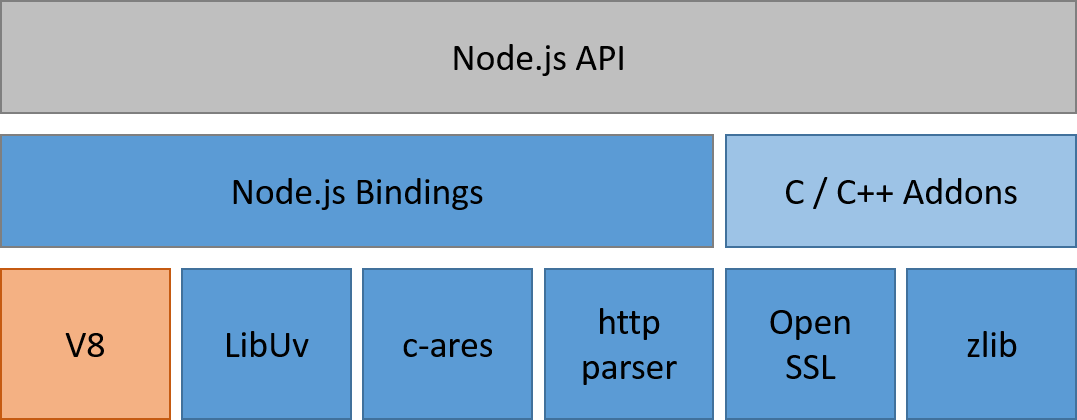
\includegraphics[scale=0.7]{img/node/nodejs-arch.png}
  \caption{Architektúra Node.js platformy.}
  \label{img-node-arch}
\end{figure}

Na vrchole obrázku máme základné Node.js API. Je napísané v JavaScripte a je priamo dostupné programátorom, pre využitie v ich aplikáciach. Pod základným API je knižnica, ktorá viaže C/C++ s JavaScriptom. Node.js tiež poskytuje doplnky (addons), čo sú dynamicky linkované zdielané objekty. Tie sa viažu na C/C++ knižnice. To znamená, že môžeme využiť skoro hocijakú C/C++ knižnicu a vytvoriť z nej doplnok, ktorý použijeme v Node.js.\\
Pod týmto všetkým máme už len natívne knižnice vytvorené v C/C++:

\textbf{V8} je open source JavaScript engine, ktorý bol vytvorený pre Google Chrome. Je napísaný v C++ a je možné ho spustiť samostatne alebo v hocijakej C++ aplikácií. V podstate kompiluje JavaScript kód do natívneho strojového kódu, namiesto toho, aby bol interpretovaný.

\textbf{Libuv} je multiplatformová podporná knižnica zo zameraním na asynchónne I/O operácie. Zo začiatku Node.js začal používať \textit{libuv} ako abstrakčnú vrstvu pre \textit{libev} a \textit{libio}, ale neskôr sa libuv stala robustnejšou a nahradila túto funkcionalitu, aby sa mohla stať multiplatformovou. Keď V8 spravuje vykonávanie JavaScriptu, tak libuv spravuje udalostnú slučku (event loop) a asynchrónne I/O operácie.
V tomto zozname vidíme všetky možnosti \textit{libuv}:
\begin{itemize}
\item plnohodnotnú údalostnú slučku, ktorú tvorí epoll, kqueue, IOCP a udalostné porty,
\item asynchronné TCP a UDP sockety,
\item asynchronné DNS,
\item asynchronné operácie nad súbormy a súborovým systémom,
\item udalosti nad súborovým systémom,
\item preklad ANSI kódov kontrolovaných cez TTY,
\item IPC so zdielaním socketu s využitím Unix socketov alebo pomenované kanály (Windows),
\item detské procesy,
\item vlákna a synchronizáciu,
\item riadenie signálov,
\item hodiny s presným časovaním (hight resolution clock).
\end{itemize}

\textbf{c-ares} je C knižnica pre asynchronné DNS žiadosti vrátane prekladanie názvov. Je určená pre aplikácie, ktoré potrebujú vykonávať dotazy na DNS bez blokovania, alebo je potrebné vykonať niekoľko dotazov paralerne.

\textbf{http\_parser} je parser pre požiadavky a odpovede  HTTP napísaný v C. Nerobí žiadne systémové volania ani alokácie, neukladá dáta do vyrovnávacej pamäte, môže byť zrušený okamžite. Jeho hlavné vlastnosti sú:
\begin{itemize}
\item žiadne závislosti,
\item udržiava trvalý stream
\item dekódovanie blokového kódovania,
\item chráni buffer proti útokom.
\end{itemize}

\textbf{OpenSSL} je open source implementácia SSL v2/v3 a TLS v1 protokolov ako aj kryptografickú knižnicu pre všeobecné účely. Je založená na SSLeay knižnici. Tá poskytuje všetky potrebné kryptografické metódy ako je hash, hmac, cipher, decipher, sign a verify metódy.

\textbf{Zlib} je všeobecná knižnica na kompresiu dát napísaná v C.\cite{nodejs-arch}


\subsubsection{Event loop}
Udalostná slučka dáva Node.js možnosť zvládnuť veľké množstvo súčasných požiadaviek aj keď je spustený v "jednom vlákne". V každej udalostne riadenej aplikácií je vo všeobecnosti hlavná slučka ktorá počúva a čaká na udalosti a keď udalosť je zaregistrovaná tak sa zavolá callback funkcia. Na obrázku č.\ref{img-node-event-loop} je zjednodušený pohľad na to, ako to funguje vrámci Node.js.

\begin{figure}[H]
  \centering
  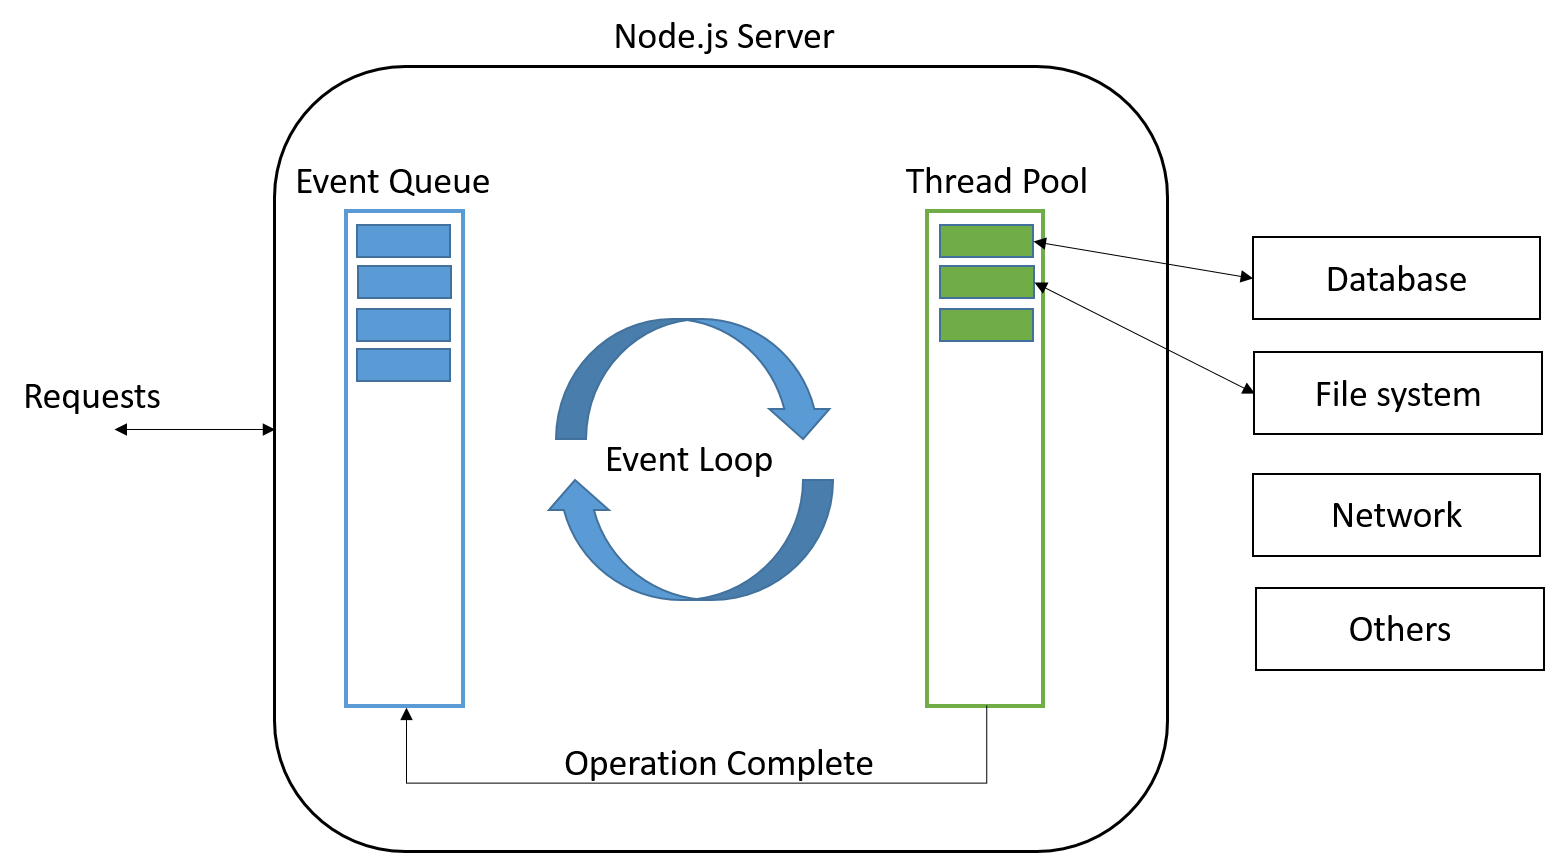
\includegraphics[scale=0.6]{img/node/nodejs-event-loop.png}
  \caption{Udalostná slučka.}
  \label{img-node-event-loop}
\end{figure}

Udalostná slučka jednoducho prechádza cez frontu čo je vlastne zoznam udalostí a callbackov vykonaných operácií. Všetky I/O operácie sú vykonané asynchrónne vláknami vo "vláknovom stacku" (thread pool). Tu zohráva dôležitú rolu libuv. Ak nejaká položka vyžaduje I/O operáciu, tak udalostná slučka jednoducho prenechá operáciu do vláknového stacku. Udalostná slučka pokračuje vo vykonávaní položiek v udalostnej fronte. Keď je I/O operácia hotová, tak callback je zaradený na spracovanie. Udalostná slučka vykoná callback a poskytne požadované výstupy. A takto sa celý proces opakuje.\cite{nodejs-event-loop}

\subsubsection{Možnosti a využitie}
Na základe popísaných základných častí Node.js v predchádzajúcich sekcií si ukážeme možnosti využitia, resp. výhody a nevýhody.\cite{nodejs-arch}

\textbf{Výhody}
\begin{itemize}
\item asynchrónne I/O - vhodné pre webové a sieťové aplikácie,
\item rôzne možnosti škálovania,
\item programovací jazyk je JavaScript, čiže rovnaký jazyk aj pre backend aj fronend,
\item jednoducho je možné s nim začať na rozdiel od Javy alebo .NET, stačí len zmeniť myslienie na asynchrónne,
\item veľmi aktívna komunita, ktorá zdieľa množstvo kódu na verejných repozitároch ako github,
\item rýchlo rastúca NPM komunita s množstvom modulov pripravených na použitie.
\end{itemize}

\textbf{Nevýhody}
\begin{itemize}
\item veľmi neefektívne pre ukóny náročné na CPU, ako generovanie reportov, analýzy, výpočty...
\item použitím udalosťami riadenej metodológie bez pochopenia prístupu môže viesť k nevhodne napísaným kódom (napr. "callback hell"),
\item neexistuje veľa štandardných knižníc ako pri Java, .NET platforme ako sú napr. XML parsery, alebo zložitejšie dátové štruktúry.
\end{itemize}

Teda Node.js nie je vhodný na všetko, vždy záleží od konkrétnej potreby. Čiže ak potrebujeme streaming alebo rýchly upload súborov, real-time údaje, single page aplikácie, websockety tak je na takéto úlohy vhodný. Vo všeobecnosti všade kde sa používa I/O operácie, tak vie zvládnuť veľké množstvo súčasných spojení.\cite{nodejs-introduction}

\subsection{Node Package Manager}
Node.js po nainštalovaní obsahuje aj \textit{NPM} (Node Package Manger). NPM je program, ktorý sa spúšta z príkazového riadku, pomocou ktorého vieme sťahovať moduly z centrálneho repozitára (\textit{https://www.npmjs.org}). Rovnako aj môžme vytvoriť vlastný modul a uložiť ho do repozitára.\\
Každý modul by mal mať vlastný adresár, ktorý tiež obsahuje súbor s metadátami volaný \textit{package.json}. V tomto súbore musí byť nastavené aspoň tieto dve vlastnosti: \textit{name, version}.\cite{nodejs-by-example}

\begin{figure}[H]
  \centering
  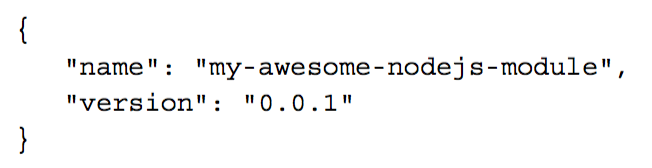
\includegraphics[scale=0.7]{img/npm/npm-minimum.png}
\end{figure}

\subsubsection{Použitie modulov}
Vo všeobecnosti sú tri možnosti ako použiť moduly, ktoré už existujú. Všetky tri zahŕňajú manažéra na spravovanie balíkov:\cite{nodejs-by-example}
\begin{itemize}
\item môžme nainštalovať špecifický modul manuálne tak, že sa presunieme do požadovaného priečinka a zavoláme v termináli 
\textit{npm install nazov-modulu}
Správca balíkov automaticky nainštaluje poslednú verziu modulu a vloží ju do priečinka \textit{node\_modules}. Ak ho chceme použiť, nepotrebujeme volať celú cestu, ale len \textit{require(nazov-modulu)}.
\item inštalácia modulu globálne vďaka \textit{-g} značke v príkaze.
\textit{npm install nazov-modulu -g}
Je to vhodnejšie používať skor na vývojové nástroje ako na bežné moduly.
\item posledná možnosť je zavolanie
\textit{npm install}
nad priečinkom kde sa nachádza už predtým spomínaný \textit{package.json} a obsahuje v sebe vlastnosť \textit{dependencies}
\end{itemize}

\begin{figure}[H]
  \centering
  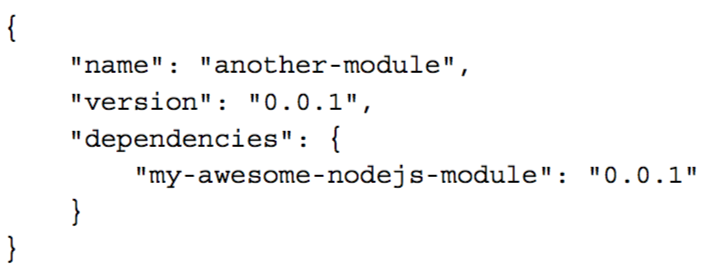
\includegraphics[scale=0.7]{img/npm/npm-overview-dependency.png}
\end{figure}

\subsubsection{Vstavané moduly}
Node.js je považovaný za technológiu, pomocou ktorej môžeme tvoriť backend aplikácie. Často potrebujeme robiť rôzne úlohy. V Node.js existujú veľmi nápomocné moduly, ktoré môžeme využiť.\cite{nodejs-by-example}

\subsubsection{Vytvorenie web servera pomocou HTTP modulu}
Modul \textit{http} patrí medzi veľmi používané, pretože vďaka nemu spustíme web server na konkrétnom porte.

\begin{figure}[H]
  \centering
  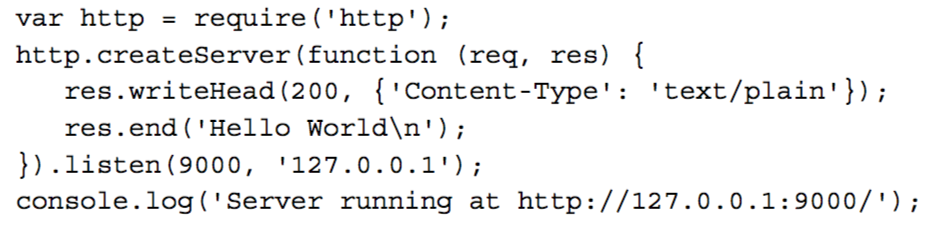
\includegraphics[scale=0.7]{img/npm/npm-http-module.png}
\end{figure}

Máme dostupnú metódu \textit{createServer}, ktorá vracia nový web server objekt. Vo väčšine prípadov zavoláme aj metódu \textit{listen}. Ak je potrebné tak pomocou \textit{close} zastavíme prímanie nových požiadaviek. Callback funkcia, ktorú tam využívame, vždy má \textit{request} (req) a \textit{response} (res) objekty. Prvý objekt môžeme použiť na získanie informácií o prichádzajúcich požiadaviek ako napr. \textit{GET}, \textit{POST} parametre.\cite{nodejs-by-example}

\subsection{Express.js}

\subsection{MongoDB}
MongoDB je multi platformová dokumentovo orientovaná databáza. Je klasifikovaná ako NoSQL databáza, čiže nepoužíva klasickú štruktúru ako v relačnej databáze na báze tabuliek, ale objekty vo forme JSON dokumentov s dynamickými schémami (v MongoDB sa volá tento formát BSON). Vďaka ukladaniu JSON dokumentov je možné ukladať dáta z rôznych aplikácií rýchlejšie a jednoduchšie.\cite{mongodb-wiki}

\begin{figure}[H]
  \centering
  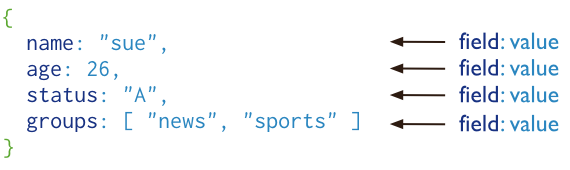
\includegraphics[scale=0.7]{img/mongodb/crud-annotated-document.png}
  \caption{JSON dokument v MondoDB.}
  \label{mongodb-example}
\end{figure}

Na obrázku č.\ref{mongodb-example} je príklad dokumentu, ktorý sa ukladá do MongoDB, v jednoduchých prípadoch nie je vidieť žiadny rozdiel oproti klasickému JSON.

\subsection{Angular.js}
Angular.js, bežne označovaný aj ako Angular je open-source framework pre web vytvorený Slovákom Miškom Hevery do verzie 1.0. Neskôr vývoj a údržbu frameworku vzal pod seba Google. Bol vytvorený za účelom tvorby SPA (single page applications), čiže webových aplikácii, v ktorých je možné aktualizovať svoj obsah bez toho, aby si užívateľ toho vo väčšej miere všimol. Cieľom je zjednodušiť vývoj, ale aj testovanie front-end web aplikácií na báze MVC (model-view-controller) alebo MVVM (model-view-view-model) architektúre.
Angular.js framework funguje tak, že pri prvom načítaní HTML stránky vloží k elementom vlastné atribúty. Angular interpretuje tieto atribúty ako direktívy a viaže ich vstupno-výstrupné časti ako model, ktorý je reprezentovaný štandardnými premennými JavaScriptu. Hodnoty týchto premenných môžu byť manuálne nastavené v kóde, alebo získané z statických (väčšinou uložené na súborovom systéme), dynamických (získané z RESTful služby) JSON súborov.
Je front-end súčasť MEAN vývojarského stacku, čo je vlastne \textbf{M}ongoDB databáza, \textbf{E}xpressJS web server framework, \textbf{A}ngular  a \textbf{N}odeJS ako aplikačný server, resp. prostredie.\cite{angular-wiki}\cite{angular-docs}

\subsubsection{Koncept}
Angular teda ako framework sa skladá z viacerých časti, ktoré robia svoju časť práce. Na obrázku je možné vidieť jeho základné komponenty, z ktorých sa skladá. Nižšie si popíšeme hlavne tie, ktoré využívame v práci.\cite{angular-concept}

\begin{figure}[H]
  \centering
  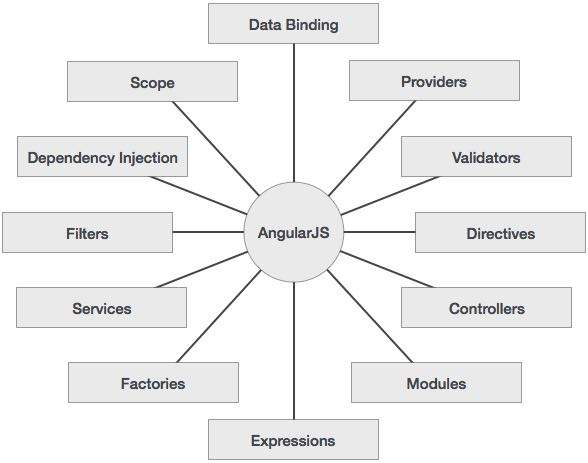
\includegraphics[scale=0.5]{img/angular/angularjs_concepts.jpg}
  \caption{Koncept frameworku Angular.js.}
  \label{img-angular-concept}
\end{figure}

\textbf{Directives}\label{angular-directives}
Jednoducho povedané, directívy sú značky na DOM elemente (napr. atribút, element, komentár alebo CSS trieda), ktorá povie Angular HTML compileru (\textit{\$compile}), aby priradil špecifické správanie na daný DOM element (napr. pomocou event listenerov), alebo dokonca transformoval DOM element ako svoje dieťa. V šablónach sa spájajú informácie z modelu a controlleru pre renderovanie dynamického obsahu, ktorý potom vidí užívateľ v prehliadači.
Angular je dodávaný zo vstavanými directivámi, od ktorých sa očakáva, že budú využívané často. Napr. \textit{ngBind}, \textit{ngModel}, \textit{ngClass}.\cite{angular-docs}

\subsubsection{Scope}
Scope je objekt, ktorý odkazuje na model aplikácie. Je to kontext, na ktorom sa vykonávajú výrazy. Scopes sú usporiadané do hierarchickej štruktúry, ktorá napodobňuje DOM štruktúru aplikácie. V scope je možné sledovať model pomocou  textit{\$watch} a vykonávať udalosti (\textit{\$apply}) cez celý systém do view. Je považovaný ako lepidlo medzi aplikačným controllerom a view. Aj controller aj directivy majú prístup k scope, ale nie navzájom k sebe. Vďaka tomu je controller izolovaný od directivy a tak isto aj od DOM. 
Každá aplikácia ma práve jeden \textit{\$rootScope}, ale môže mať viacero detských \textit{\$scope}. Aplikácia môže mať viacero scopes, pretože niektoré directívy môžu vytvoriť nový detský scope, ak to potrebujeme. Keď je nový scope vytvorený, tak je priradený ako dieťa k rodičovskému scope. Toto vytvára stromovú štruktúru paralernú k DOM, kde sú priradené.\cite{angular-docs}

Dirty checking v scope pre zmeny vlastností objektu je často používaná operácia a preto by mala byť efektívna. V závislosti od potreby môže byť dirty checking využité týmito troma stratégiami: referenciou na objekt, obsah poľa alebo na hodnoty objektu. Líšia sa v spôsobe zaregistrovania zmeny aj výkonostnými rozdielmi.


\begin{itemize}
  \item Sledovanie podľa referencie \textit{\$scope.\$watch(watchExpression, listener)}: detekuje zmenu, keď sa do sledovanej hodnoty nastaví nová. Ak sledovaný objekt, alebo pole, zmeny vnútri nie su detekované. Toto je najúčinnejšia stratégia.
  \item Sledovanie na celej kolekcii (poli) \textit{\$scope.\$watchCollection(watchExpression, listener)}: detekuje zmeny, ku ktorým dochádza vo vnútri poľa alebo objektu. Napr. keď sú položky pridané, odstránené alebo sa v nich zmenilo poriadie. Detekcia je plytká, čiže nesleduje vnorené kolekcie. Sledovanie celého obsahu kolekcie je výkonovo náročnejsie ako sledovanie podľa referencie, pretože treba uchovávať kópie obsahu. Avšak, táto stratégia sa snaží minimalizovať množstvo potrebných kopírovaní.
  \item Sledovanie všetkých položiek objektu \textit{\$scope.\$watch(watchExpression, listener, \textbf{true})}: detekuje akúkoľvek zmenu v ľubovolnej vnorenej štruktúry. Táto stratégia má najväčšie možnosti detekovania zmien, ale za to aj výkonovo a pamäťovo náročnejšia. Je potrebné uchovávať kópiu celej vnorenej štruktúry a pri každej zmene, sa musí nakopírovať do pamäte.
\end{itemize}

\begin{figure}[H]
  \centering
  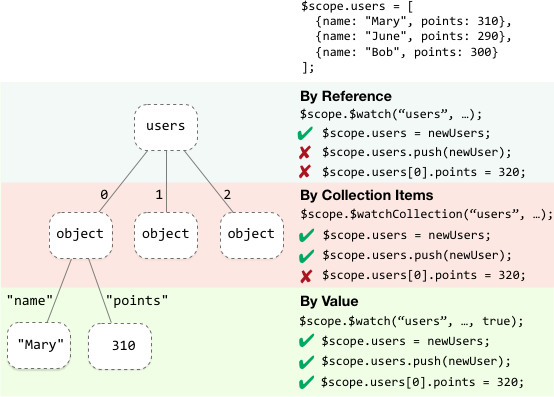
\includegraphics[scale=0.7]{img/angular/concepts-scope-watch-strategies.png}
  \caption{Možnosti sledovania modelu v Angular.js.}
  \label{img-angular-watchl}
\end{figure}

\subsubsection{Expressions}
Angular výrazy sú kúsky kódu v JavaScripte, ktoré sú umiestnené medzi dvojitými kučeravými zátvorkami. Príklad: \textit{<span title="\textbf{\{\{} attrBinding \textbf{\}\}}">\textbf{\{\{} textBinding \textbf{\}\}}</span>}. Vyhodnotenie môže rovnako prebehnúť aj vo funkcii na kliknutie \textit{ng-click="functionExpression()"}.
Pre príklad pridávam zopár ďalších platných výrazov, ktoré sa často môžu používať: \textit{\{\{ 1 + 2 \}\}}, \textit{\{\{ a + b \}\}}, \textit{\{\{ user.name \}\}} a 
\textit{\{\{ items[index] \}\}}.\cite{angular-docs}

%\textbf{Compiler}

%\textbf{Filter}

%\textbf{View}

\subsubsection{Data Binding}
Data binding v Angulare funguje ako automatická synchronizácia dát medzi modelom a view. Ak sa zmení model, tak zmena sa automaticky prejaví aj do view, alebo aj naopak.
Na obrázkoch môžeme vidieť pre porovnanie aký je rozdiel medzi One-way a Two-way data binding.

\begin{figure}[H]
\subfigure[One-way data binding]{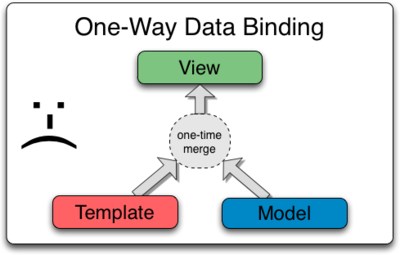
\includegraphics[scale=0.55]{img/angular/One_Way_Data_Binding.png}\label{img-angular-onedb}}
\subfigure[Two-way data binding]{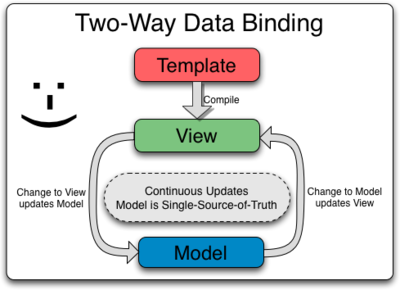
\includegraphics[scale=0.55]{img/angular/Two_Way_Data_Binding.png}\label{img-angular-twodb}}
\caption{Data binding v Angular.js.}
\end{figure}

Mnoho šablónovacích enginov nastavujú dáta len v jednom smere: spoja spolu šablónu a komponenty modelu do view. Keď sa dokončí spojenie, zmeny v modeli alebo jeho príslušných sekcií vo view sa neprejavujú automatický v zobrazení. Horšie je, že zmeny ktoré úžívateľ v zobrazení sa neprejavia do modelu. To znamená, že vývojár musí napísať kód, ktorý sústavne synchronizuje view s modelom a model s view.

Šablóny v Angulari fungujú inak. Šablóna (čo je neskompiloný HTML kód spolu s ďalšími značkami a directívami) je najprv kompilovaná v browseri. Tento krok produkuje živý view. Akékoľvek zmeny vo view sa okamžite prejavia v modeli, a akékoľvek zmeny v modeli sú poslané do view. Vďaka tomuto spôsobu môžeme o view hovoriť ako o okamžitej projekcii modelu.

Pretože view iba je projekcia modelu, tak controller je kompletne separovaný od view a nevedia o sebe. Vďaka tomu je testovanie jednoduchšie, pretože je možné testovať controller izolovane od view.\cite{angular-docs}

\subsubsection{Controller}
V Angulare je controller definovaný funkciou konštruktoru JavaScriptu, ktorý je používaný pre rozšírenie Angular Scope.
Keď je controller pripojený k DOM cez \textit{ng-controller} directívu, tak bude vytvorená inštancia objektu konštruktora. Bude vytvorený detský Scope a je dostupný ako parameter to konštruktorovej funkcie controlleru ako \textit{\$scope}.
Vo všeobecnosti by controller nemal toho robiť veľa. Mal by obsahovať iba business logiku potrebnú pre jednotlivý view. Najlepší spôsob ako zachovať controller čo najmenší, je zabalenie niektorej úlohy do service, ktorá tam nepatrí. Potom tieto úlohy zo services voláme v controlleri ako závislosť.\cite{angular-docs}\\

Controller je možné používať na:
\begin{itemize}
\item nastavenie počiatočného stavu v \textit{\$scope} objekte.
\item pridanie vlastností a správania do \textit{\$scope} objektu.
\end{itemize}

Nepoužívať controller na:
\begin{itemize}
\item manipuláciu s DOM, pretože controller by mal obsahovať iba business logiku. Vložením hociakej prezentačnej logiky do controlleru vo veľkej miere ovplyvňuje jeho testovanie. Na manipuláciu slúžia directívy v sekcii \ref{angular-directives}.
\item formátovanie vstupu - použite angular from controls
\item filtrovanie výstupu - použite angular filter
\item zdielanie kódu alebo stavu naprieč controllermi - použite angular service
\item spracovanie životného cyklu ostatných komponentov (napr vytváranie inštancíí service).
\end{itemize}

\begin{algorithm}
\lstset{
   language=JavaScript,
   backgroundcolor=\color{lightgray},
   extendedchars=true,
   basicstyle=\footnotesize\ttfamily,
   showstringspaces=false,
   showspaces=false,
   numbers=none,
   numberstyle=\footnotesize,
   numbersep=9pt,
   tabsize=2,
   breaklines=true,
   showtabs=false,
   captionpos=b
}
\begin{lstlisting}
var myApp = angular.module('myApp',[]);

myApp.controller('LabController', ['$scope', function($scope) {
  $scope.name = 'StarkLab!';
}]);

-----------------------------------------------------------------------

<div ng-controller="LabController">
  {{ name }}
</div>
\end{lstlisting}
 \caption{Ukážka controlleru v Angular.js a jeho volanie na HTML elemente.}
 \label{angular-controller}
\end{algorithm}

%\textbf{Dependency Injection}

\subsubsection{Module}
Module môžeme uvažovať ako kontainer pre rozličné časti našej aplikácie - controller, service, filter, directivy... Každý modul môže obsahovať zoznam iných modulov ako svoju závislosť. Keď závisíme na nejakom module, tak tento modul musí byť načítaný ešte pred našim modulom. Toto poriadie môžme manuálne nastaviť v konfigurácií modulov. Každý modul môže byť načítaný iba raz aj keď na ňom závisí viacero modulov.\cite{angular-docs}\\
Pri programovaní modulov musíme dávať pozor na to, aby sme si neprepísali existujúci v pamäti.

\begin{algorithm}
\lstset{
   language=JavaScript,
   backgroundcolor=\color{lightgray},
   extendedchars=true,
   basicstyle=\footnotesize\ttfamily,
   showstringspaces=false,
   showspaces=false,
   numbers=none,
   numberstyle=\footnotesize,
   numbersep=9pt,
   tabsize=2,
   breaklines=true,
   showtabs=false,
   captionpos=b
}
\begin{lstlisting}
var myModule = angular.module('myModule', []);

// pridanie directivy a sluzby do modulu
myModule.service('myService', ...);
myModule.directive('myDirective', ...);

// toto volanie prepise uz vytvorene myService a myDirective vytvorenim noveho modulu
var myModule = angular.module('myModule', []);

// vyhodi chybu pretoze volame myOtherModule, ktory este nebol definovany
var myModule = angular.module('myOtherModule');
\end{lstlisting}
 \caption{Ukážka vytvorenia modulov a pridávania funkcionality do nich.}
 \label{angular-module}
\end{algorithm}

\subsubsection{Service}
Angular service je nahraditeľný objekt, ktorý je možné použiť v aplikácií pomocou dependency injection (DI). Services môžeme použiť pre lepšiu organizáciu a zdieľanie kódu naprieč celej aplikácie. Framework poskytuje mnoho užitočných services, ako napr. \textit{\$http}, ale väčšina aplikácií má potrebu si vytvoriť vlastné.\cite{angular-docs}
Poznáme dva typy services:
\begin{itemize}
\item lazily instantiated - angular vytvorí inštanciu service iba v prípade, že na nej závisí komponent/modul
\item singleton - každý komponent závisiaci na na service získa referenciu na jedinú inštanciu generovanú z service factory.
\end{itemize}

%\subsubsection{Scope}
\subsubsection{Bootstrap aplikácie}
mozno lepsie pred konceptom
%\subsubsection{Two-way data binding}

\section{Návrh a implementácia StarkLab}
\indent Témou práce je navrhnúť a implementovať virtuálne laboratórium s využiťím JavaScriptu na strane servera. V tejto kapitole si ukážeme predpokladaný návrh celého virtuálneho laboratória s využitím technológií na jednotlivých komponentoch. Ich presný popis a využitie si popíšeme viacej v sekcii č.\ref{used-technologies}. Teda máme dané, že budeme využívať Node.js technológiu ako server. To je náš centrálny server (ďalej len StarkLab), ktorý spracováva dáta z Matlab workspace. Do Matlab workspace sú dáta posielané intervalovo zo Simulinku, v ktorom bola spustená referenčná schéma generujúca dáta. Zo začiatku nebolo isté či bude možné docieliť spustenie Simulinku v reálnom čase multiplatformovo. Našli sme riešenie Simulink Real-time priamo od Mathworks, ktorá toto umožnuje ale bohužial len pre operačný systém Windows. Lenže neskôr sme našli knižnicu \textit{tos\_lib.mdl}, ktorá nám túto funkcionalitu poskytla aj pod MAC OS X.\\
Na komunikáciu s workspace využívame volanie RESTful služieb, ktoré podporuje aj Matlab R2015b \cite{matlab-restful}. Keď si užívateľ spustí simuláciu cez klienta, tak sa údaje budú uchovávať v databáze mongoDB pre neskoršie spracovanie.

\begin{figure}[H]
  \centering
  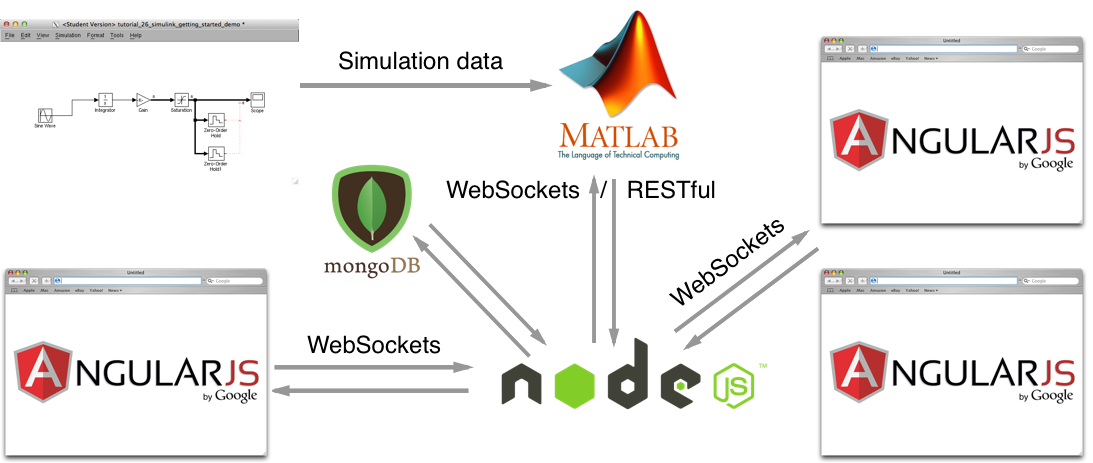
\includegraphics[scale=0.4]{img/software-design.png}
  \caption{Návrh komunikácie medzi jednotlivými komponentami.}
  \label{img-software-designl}
\end{figure}

\subsection{Referenčný model simulácie v Matlabe}
Systém síce bude mať možnosť spolupracovať s reálnymi zariadeniami, pre vývoj sme použili simuláciu dynamického systému šikmého vrhu. Pre spustenie simulácie je potrebné zavolať dva súbory. Účel prvého je inicializácia premenných potrebných pre výpočet súradníc polohy bodu v šikmom vrhu. Na obrázku č.\ref{img-matlab-function} si všimnime, že je potrebné zadať aj parametre pre spustenie a funkcia nič nevracia. Prvý z parametrov \textit{v0} nastavuje počiatočnú rýchlosť telesa v metroch za sekundu, akou bude vymrštené z bodu (0,0). Druhý parameter \textit{alfa\_deg} zase určuje pod akým uhlom bude teleso vymrštené v stupňoch. Posledný parameter \textit{runBy} nie je potrebný k samotnej simulácií, ale skôr k identifikácií, kto spustil simuláciu. Vďaka tomu je možné neskôr z databázy zistiť kto spustil simuláciu.

Keď sú parametre funkcie správne zadané a spustí sa telo funkcie, tak sa nastavia a vypočítajú hodnoty ako \textit{alfa\_rad, td, d, h} ktorých popis vidíme na obrázku a sú potrebné ako vstupné parametre do simulácie.

Posledná časť kódu od riadku č. 23 slúži pre prekopírovanie premenných do hlavného scope matlabu, čiže workspace. Keby toto neurobíme, tak všetky hodnoty po skončení funkcie zaniknú keďže sa berú ako lokálne. Síce by bolo možné sa tomuto vyhnúť, tak že by sme nevolali funkciu \textit{Sikmy\_vrh\_par(80, 70, 'xstark')} a volali len súbor, čo by vlastne zostali všetky hodnoty v hlavnom workspace. Lenže v tomto prípade by nebolo možné nastavovať inicializačné premenné z webovej aplikácie, ale by museli byť natvrdo nastavené v kóde matlabu.

\begin{figure}[H]
  \centering
  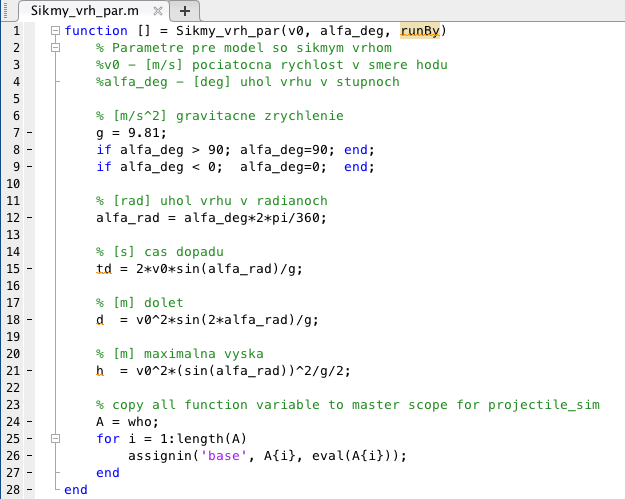
\includegraphics[scale=0.7]{img/code/matlab-function.png}
  \caption{Inicializačná funkcia šikmého vrhu v Matlabe.}
  \label{img-matlab-function}
\end{figure}

Ako sme si už povedali, že hodnoty sa po spustení úspešne uložia do Matlab workspace a to vidieť aj na obrázku č. \ref{matlab-function-workspace}. Tieto hodnoty boli vygenerované po zavolaní funkcie zo špecifickými hodnotami parametrov \textit{Sikmy\_vrh\_par(80, 70, 'xstark')}.

\begin{figure}[H]
  \centering
  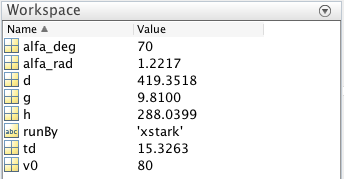
\includegraphics[scale=0.7]{img/code/matlab-function-workspace.png}
  \caption{Hodnoty v Matlab workspace po spustení funkcie.}
  \label{matlab-function-workspace}
\end{figure}

Druhý súbor, ktorý potrebujeme spustiť po tomto je obslužný kód, vďaka ktorému vieme zaslať údaje do Node.js. Kvôli jeho dĺžke a vlastnej implementácii ho nie je možné zobraziť celý, tak si popíšeme len kľúčové vlastnosti.

Pri inicializácií sa nastavi URL cesta pre Express.js API, na ktorú ma komunikovať. Prednačítavanie modelu sa vykoná pomocou funkcie \textit{load\_system('Sikmy\_vrh\_2');}. Táto funkcia vyhladá v aktuálnom priečinku súbor \textit{Sikmy\_vrh\_2.mdl} a nastaví ho ako bdroot čo je aktuálne top-level model. Po nastavení musíme simuláciu aj spustiť. Ovládanie simulácie sa robí pomocou príkazu \textit{set\_param(model, 'SimulationCommand', 'Start');}, kde posledný parameter znamená spustenie simulácie.
Následne sa spustí nekonečný \textit{while} cyklus, vďaka ktorému je možné zbierať údaje zo simulácie až do stavu kým nie je ukončená. 
Na začiatku cyklu sa volá \textit{set\_param(bdroot, 'SimulationCommand', 'WriteDataLogs');} čo vlastne pristúpi k aktuálne najvyššie spustenej simulácií a snaží sa zapísať do Matlab workspace aktuálne vypočítane hodnoty. Bez tohto príkazu by sa zapísali až po skončení simulácie.

Medzitým sa údaje upravujú na potrebný formát a pred odoslaním na REST API je vhodné ho zabaliť do JSON štruktúry. Tú vieme vytvoriť pomocou knižnice \textit{jsonlab} v aktuálnej verzií 1.2.
Pomocou sekvencie týchto dvoch príkazov vytvoríme požadovaný JSON formát a odošleme ho na API. Vytvorenie JSON \textit{json = savejson('result', struct('user', runBy, 'status', 'running', 'sessionId', 'xxx72', 'data', struct('time', A, 'vy', B, 'y', C, 'x',D)));} a zaslanie do služby \textit{response = webwrite(url,json,options);}. Pomocou príkazu \textit{get\_param(model, 'SimulationStatus')} vieme získať aktuálny stav simulácie. V prípade, že simulácia stále beží tak získame výstup \textit{'running'} inak je ukočená a vráti reťazec \textit{'stopped'}. Hneď ako dostaneme status 'stopped' tak ukončíme cyklus pomocou \textit{break} a vieme že všetky dáta su prenesené do Node.js.

\subsection{Diagramy}
Diagramy su sucastou sytemu .....

\subsubsection{Prípad použitia}
Na obrazku ...

\begin{figure}[H]
  \centering
  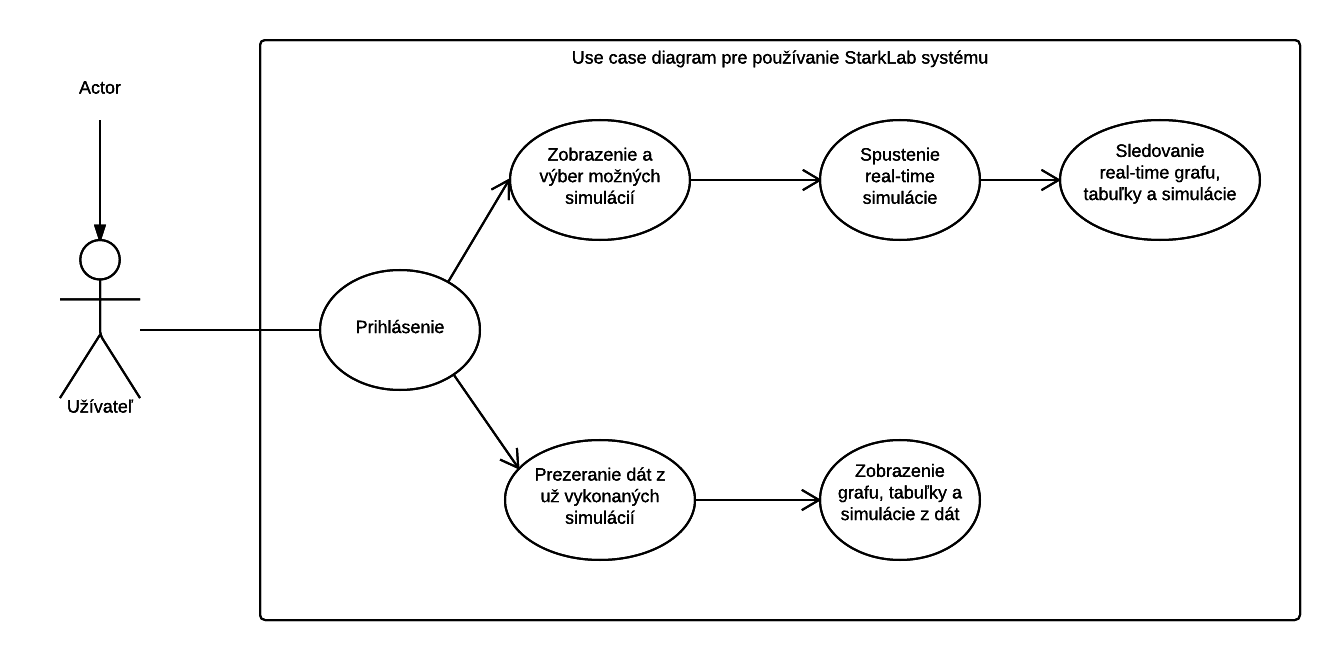
\includegraphics[scale=0.7]{img/diagrams/use-case.png}
  \caption{Diagram prípadu použitia na prácu zo systémom.}
  \label{img-use-case}
\end{figure}

popis tohto pripadu, mozno z tabulky na ceskom webe alebo vseobecne


\subsubsection{Sekvenčný diagram}\label{diagram-sequence-section}

\begin{figure}[H]
  \centering
  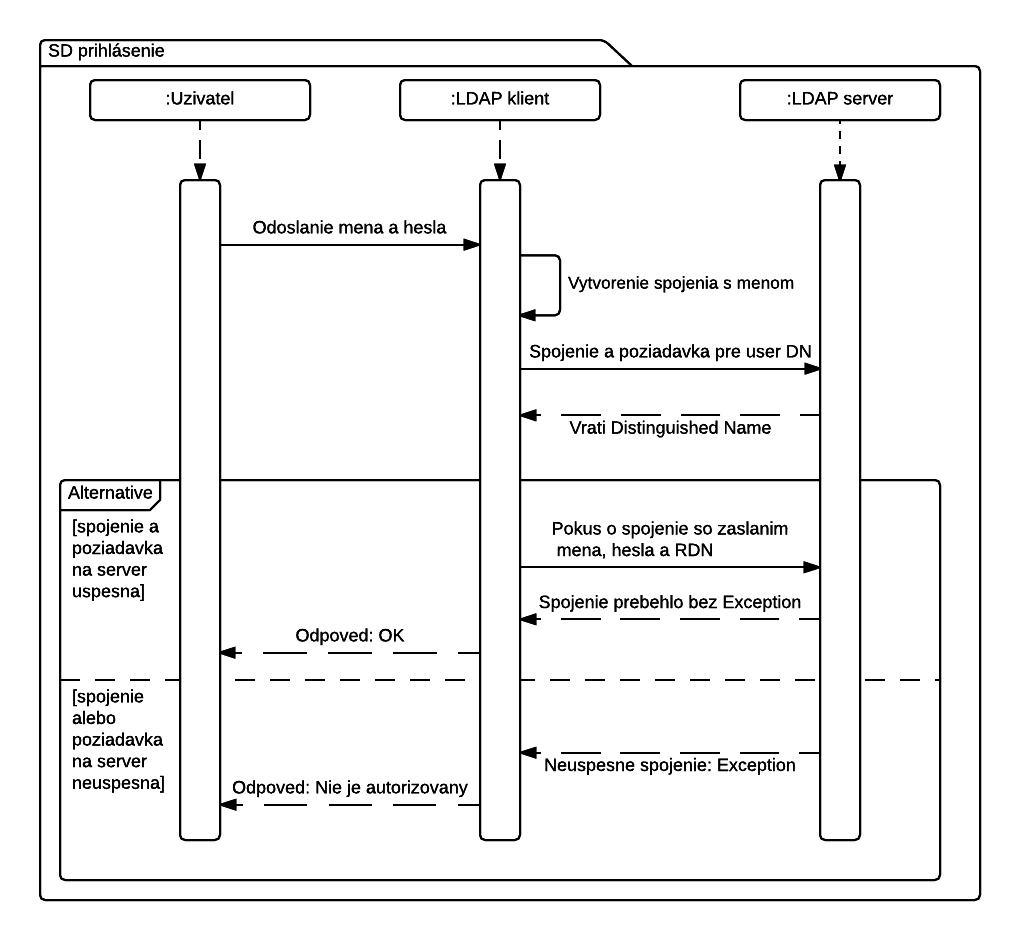
\includegraphics[scale=0.7]{img/diagrams/sequence-ldap.png}
  \caption{Sekvenčný diagram pre prihlásenie pomocou LDAP.}
  \label{img-sequence-ldap-login}
\end{figure}

Na obrázku č.\ref{img-sequence-ldap-login} si všimneme ako približne funguje prihlásenie pomocou mena a hesla do LDAP systému. Nižšie si popíšeme kód ako to máme implementované v JavaScripte. Toto je len časť kódu, ktorá sa určená pre prihlásenie do systému. Na začiatku súbotu je volaná požadovaná knižnica pre prácu s LDAP ako \textit{var ldap = require("ldapjs");}
Keď užívateľ príjde na stránku a vyplní prihlasovacie meno a heslo do stuba ldap, tak formulár ho presmeruje na \textit{/login}, kde už sa postaral o routovanie Express.js. Z \textit{request} parametra získame zadané username - \textit{req.body.username} a password - \textit{req.body.password}, ktoré sme vyplnili pred odosielaním formulára. Čiže ak sú oba vyplnené dostaneme sa do vnútra podmienky, kde sa vytvorí spojenie na linku \textit{ldap://ldap.stuba.sk}, vytvorí RDN reťazec v tvare \textit{"uid=xstark", ou=People, DC=stuba, DC=sk"}.
V momente keď je zostavený reťazec a máme získané heslo užívateľa, tak zavoláme ldap funkciu \textit{bind} s parametrami RDN a heslom. V prípade ak nenastala žiadna chyba pri overovaní, tak sme úspešne overený a vytvoríme \textit{session} a \textit{cookie} pre užívateľa a presmerujeme ho na stránku, kde už môže vidieť možné simulácie.

\begin{figure}[H]
  \centering
  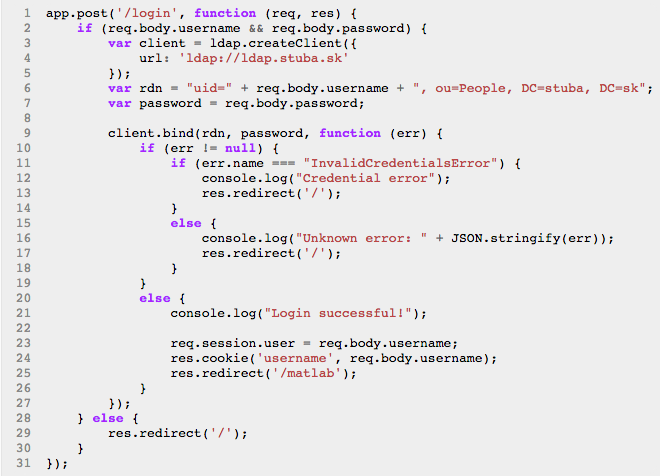
\includegraphics[scale=0.7]{img/code/ldap-login.png}
\end{figure}

\subsection{Databázový model MongoDB}
V našom zadaní sme nepoužívali štandardnú SQL databázu, čiže nie je možné využiť bežné modelovanie cez ERD diagramy. Ako už vieme MongoDB neukladá dáta ako tabuľky, ale JSON dokumenty. Keďže sa jednalo o jednoduchý model šikmého vrhu, tak v tomto prípade nebude model extra zložitý. V tejto časti si ukážeme do akého objektu ho v JavaScripte ukladáme a potom konkrétny príklad z databázy.

\begin{figure}[H]
  \centering
  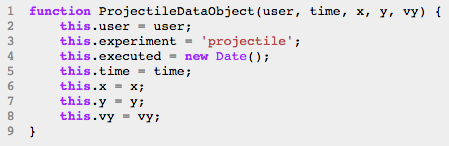
\includegraphics[scale=0.7]{img/code/javascript-projectile-model.png}
  \caption{Model objektu v JavaScripte, pre vytvorenie záznamu v MongoDB.}
  \label{img-js-projectile-model}
\end{figure}

Ako vidíme v JavaScripte sa nepoužívajú žiadne typy. Hodnoty \textit{user, experiment} budú vždy typu \textbf{\textit{String}}, \textit{executed} je typu \textbf{\textit{Date}} vo formáte ISO-8601 a jeho formát je YYYY-MM-DDTHH:mm:ss.sssZ. Zvyšok hodnôt \textit{time, x, y, vy} sú hodnoty závislé od simulácie a každá z nich je pole čísiel.

Na obrázku č.\ref{img-mongo-record} je záznam z MongoDB kde konkrétne hodnoty time, x, y, vy nie sú zobrazené, pretože simulácia vygenerovala až 788 hodnôt.

\begin{figure}[H]
  \centering
  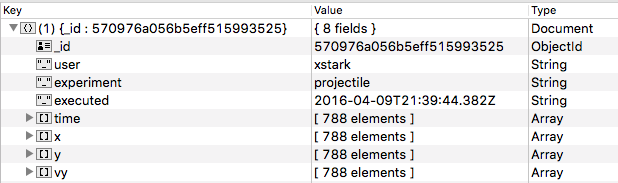
\includegraphics[scale=0.7]{img/code/mongodb-record.png}
  \caption{Príklad záznamu simulácie v MongoDB.}
  \label{img-mongo-record}
\end{figure}

%\section{Testovanie}

\subsection{Node.js s frameworkom Express.js}
Hlavná časť tejto práce je sústredená na komunikáciu medzi Matlabom a Node.js, resp Express.js. Je to vlastne len nadstavba a umožnuje jednoduchšiu tvorbu REST služieb. Na začiatok si povieme čo sme použili ako \textit{middleware}. Ako sme si už hovorili je to funkcia, ktorá má prístup do request objektu a response objektu. Použili sme \textit{body-parser}, vďaka ktorému bolo možné spracovávať telo POST požiadavky, ktorá sa zasielala z Matlabu. Potom ho je potrebné ešte aj aktivoať ako middleware v kóde \textit{app.use(bodyParser.json({limit: '2mb'}));}. Po viacerých testoch som zistil, že základný limit je nastavený na 1MB, kde sa vyskytoval problém s príjmutím POST requestu, v prípade ak boli údaje v tele moc dlhé.

\subsubsection{Vlastný middleware prihlasovania}
V aktuálnom softwarovom riešení nebolo potrebné vytvoriť prihlasovanie, pretože neskôr bude integrované do LMS Moodle, ktorý si takéto veci už rieši svojím spôsobom. Ale pre ukážku možností frameworku Express.js som implementoval middleware \textit{express-session}, vďaka ktorému môžme vytvoriť reláciu pre úspešne autorizovaného užívateľa. 

Pri implementácii prihlasovania cez nastavovania session som zistil, že v každom smerovaní (route), bolo potrebné kontrolovať na začiatku kódu, či je prihlásený používateľ alebo či je to požiadavka z Matlab služby. Pri väčšom projekte, prípadne viacerých route by to začalo byť neefektívne a neprehľadné. Vytvorili sme vlastný middleware na obrázku č. \ref{img-express-middleware}, ktorý nam overuje prihláseného človeka pri každom prístupe na hocijakú route.

\begin{figure}[H]
  \centering
  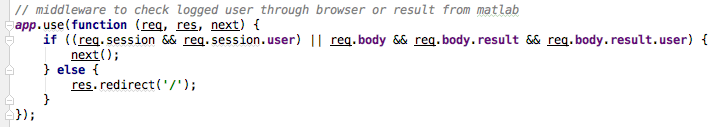
\includegraphics[scale=0.6]{img/code/express-middleware.png}
  \caption{Middleware kód v Express.js na kontrolu prihlásenia.}
  \label{img-express-middleware}
\end{figure}

Volanie \textit{app.use} nám zabezpečí, že sa táto funkcia zaregistruje ako middleware a bude volaná pri každom requeste. Prvá časť podmienky overuje, či prichádzame z webového prehliadača a je nastavená session. Kedže Matlabu nevieme nastaviť session, pretože tá sa ukladá len na webserveri tak sme to vyriešili iným spôsobom. V príchádzajúcom tele POST requestu od Matlabu je objekt \textit{result}, kde sú uložené vygenerované údaje. Priradili sme mu ďalšiu property \textit{user}, ktorá keď je nastavená, tak vieme, že požiadavka prichádza z Matlabu a vieme jej povoliť prístup. V prípade splnenej aspoň jednej podmienky sa zavolá callback \textit{next()}, čo vlastne vyvolá buď nejaký ďalší zaregistrovaný middleware, alebo route, na ktorú sme posielali požiadavku.
Ak nie je splnená ani jedna z dvoch podmienok, tak nás server presmeruje na hlavnú stránku, kde sa od nás požaduje znovu prihlásenie.


\subsubsection{Spustenie Matlabu zo Simuláciou}
Nebolo isté ako budeme spúšťať simuláciu, pretože nebolo isté či Node.js umožuje vykonávať príkazy nad operačným systémom, resp. spúšťať programy. Spočiatku sme riešili komunikáciu takým spôsobom, že Matlab sa spustil ručne a v ňom potrebné inicializačné súbory a následne samotná simulácia. Takéto riešenie nie je postačujúce z hladiska automatizácie a samostatnosti.

Potom sme zistili, že Node.js má možnosti na spustenie hocijakého software, ktorý je možné spustiť cez terminál. Pre zjednodušenie práce som využil modul \textit{shelljs}, ktorý túto funkcionalitu poskytuje. Na obrázku č. \ref{img-express-shelljs} je funkcionalita, ktorá sa vykoná po prístupe na route /matlab/run. Táto časť sa volá po odoslaní formuláru s parametrami počiatočnej rýchlosti a uhlu z webového prehliadača.

Ako vidíme vstupný reťazec, ktorý chceme vykonať, bolo potrebné zadať cestu k Matlabu kde sa nachádza na súborom systéme. Ďalej je vidieť, že sa spúšta aj s istými parametrami. Všetky potrebné možnosti som našiel v online dokumentácii Matlabu. \cite{matlab-macos}

Keďže sa spúšta z terminálu a nie je potrebné, aby nám ukazoval výsledky aj v okne, tak jeho spúštanie vieme urýchliť použitím parametrov, ktoré vidíme na obrázku. Pomocou parametra \textit{-r} vieme vykonávat príkazy v príkazovom riadku Matlabu, napr. špecifikovať cestu, kde sa nachádza naša simulácia a potrebné súbory. Následne zavoláme funkciu \textit{Sikmy\_vrh\_par()} kam sa pošlú parametre počiatočnej rýchlosti a uhla a zároveň prihlásený používateľ. Hneď ako sa skončí vykonávanie tejto funkcie, spustí sa súbor \textit{projectile\_sim} čo je už konkrétna simulácia. Po skončení už môžeme zatvoriť aj Matlab cez príkaz \textit{exit;}.

Po zostrojení tohto reťazca ako parametra funkcie \textit{exec} a jeho spustení sa čaká na vykonávanie Matlabu. Medzitým nás server presmeruje na stránku /dashboard kde sa čaká na údaje zo simulácie. Hneď ako sa načíta simulácia zo vstupými parametrami a začne vykonávať v momente sa údaje zobrazia aj vo webovom prehliadači realtime.

\begin{figure}[H]
  \centering
  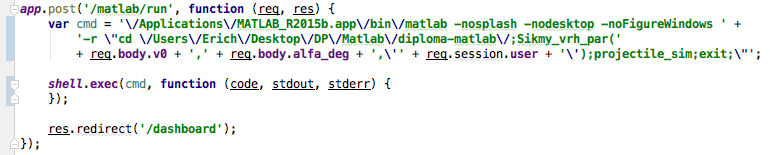
\includegraphics[scale=0.7]{img/code/express-shelljs.png}
  \caption{Spustenie príkazu v OS pomocou shelljs modulu.}
  \label{img-express-shelljs}
\end{figure}

\subsection{Webový klient s frameworkom Angular.js}
Na klientskú časť práce sme využili JavaScriptový framework Angular.js v poslednej stabilnej verzii 1.5.5. Úloha webového klienta, bolo overiť funkčnosť vytvoreného prostredia, ktorý generujé údaje. Funkčnosť sme overili a popíšeme si konkrétne obrazovky.

\begin{figure}[H]
  \centering
  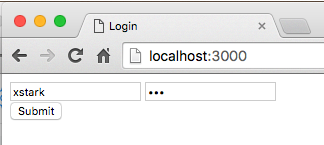
\includegraphics[scale=0.7]{img/code/angular-login.png}
  \caption{Prihlásenie do LDAP pomocou STUBA údajov.}
  \label{img-angular-login}
\end{figure}

Ako to funguje na pozadí už sme si popísali v sekcií \ref{diagram-sequence-section}, kde sa pojednávajú sekvenčné diagramy, konkrétne prihlásenie do LDAP.
Po prihlásení sa zobrazí stránka vyhradená pre zadanie parametrov šikmého vrhu, počiatočnú rýchlosť v0 a uhol vystrelenia alfa\_deg. Pri zadaní rýchlosti v0=40 a alfa\_deg=60 sme presmerovaní na stránku /matlab.

\begin{figure}[H]
  \centering
  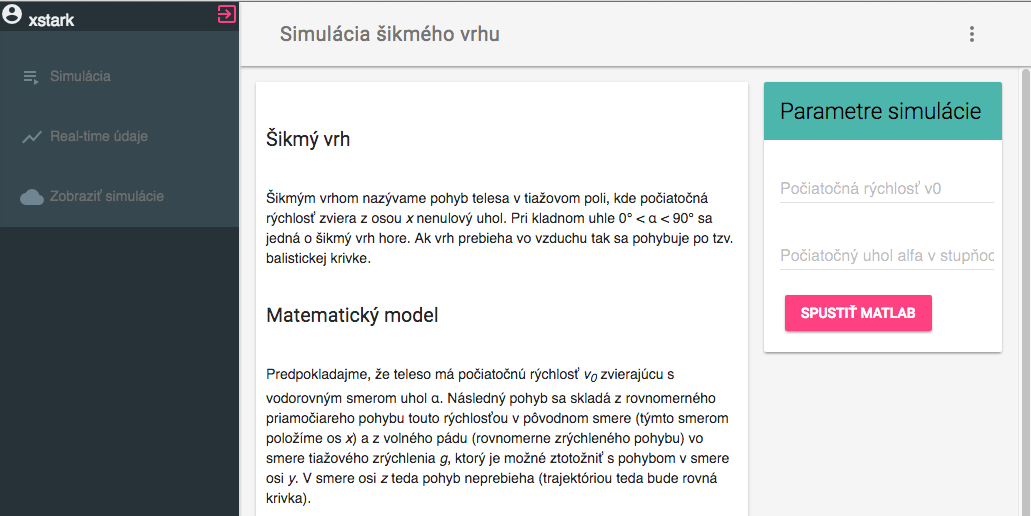
\includegraphics[scale=0.7]{img/code/angular-simulation-param.png}
  \caption{Parametre simulácie - počiatočná rýchlosť a uhol v stupňoch.}
  \label{img-angular-params}
\end{figure}


\subsubsection{Grafy s Chart.js}

Treba počkať kým sa spustí Matlab zo simuláciou a následne sa začnú generovať údaje realtime do prehliadača. Táto časť by mohla byť zrýchlená tým, že sa Matlab bude nachádzať na výkonnom serveri. Na obrázku č. \ref{img-angular-chartjs} je využitá knižnica Chart.js pre tvorbu grafov.

\begin{figure}[H]
  \centering
  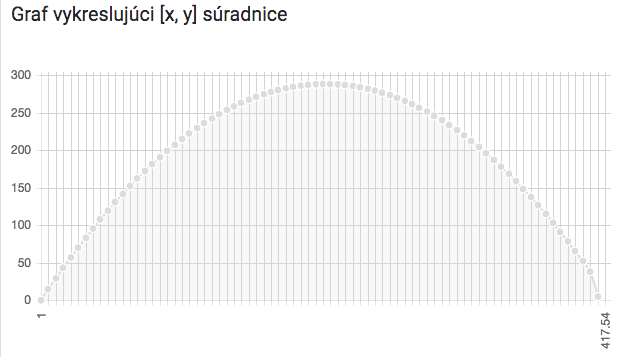
\includegraphics[scale=0.5]{img/code/angular-chartjs.png}
  \caption{Graf vykreslujúci závislosti [x, y] v šikmom vrhu.}
  \label{img-angular-chartjs}
\end{figure}

\subsubsection{Animácia pomocou html canvas}\label{section-canvas}

Na ďalšom obrázku č. \ref{img-angular-canvas} sa vykreslujú rovnaké údaje ako na grafe, len je to spôsobom animácie guličky. Táto animácia bola vytvorená pomocou html canvas technológie. Viac o canvas v sekcii \ref{section-canvas}.

\begin{figure}[H]
  \centering
  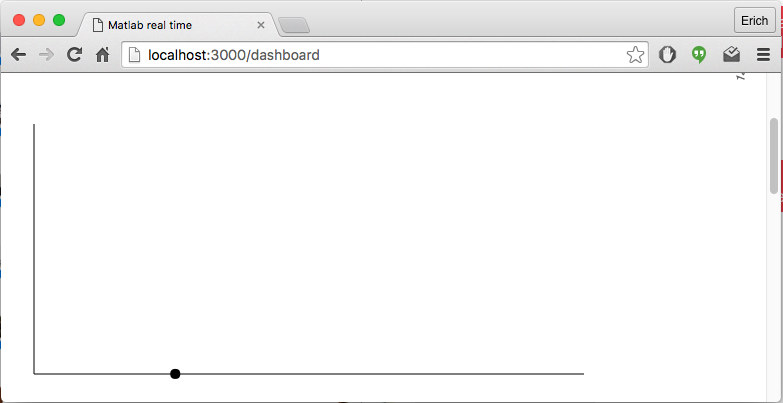
\includegraphics[scale=0.5]{img/code/angular-canvas.png}
  \caption{Animácia vykreslujúca závislosti [x, y] v šikmom vrhu.}
  \label{img-angular-canvas}
\end{figure}

\subsubsection{Tabuľka dát}

Ako posledná časť sledovania dát je tabulka, ktorej údaje sa generujú rovnako realtime ako aj pri grafe a animácii pred ním.

\begin{figure}[H]
  \centering
  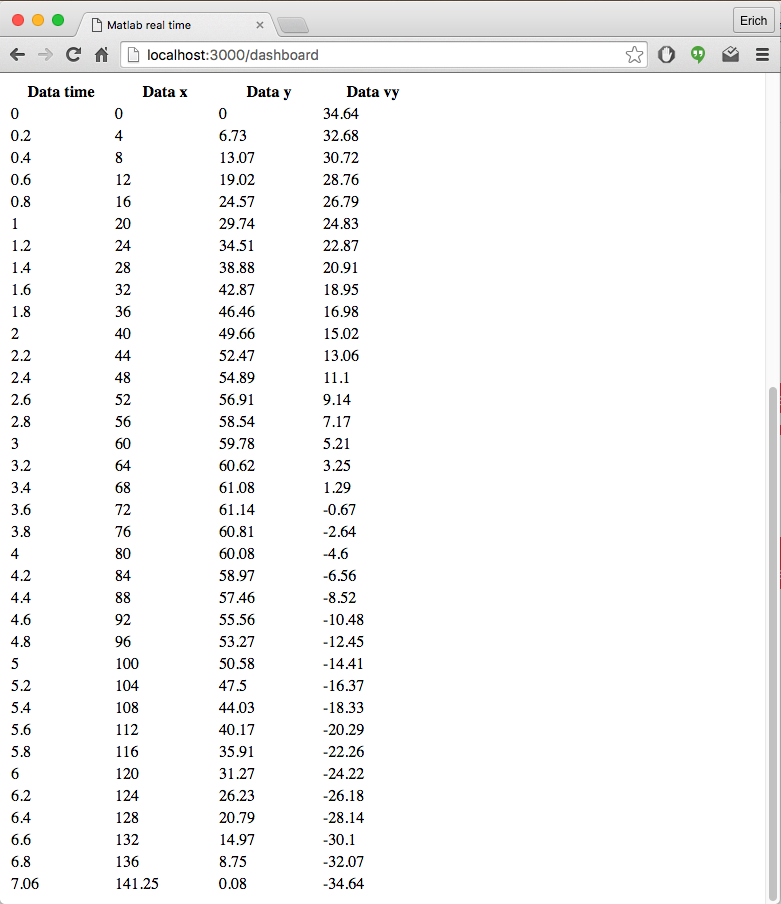
\includegraphics[scale=0.5]{img/code/angular-table.png}
  \caption{Tabuľka dát času, x, y a smer rýchlosti vy.}
  \label{img-angular-table}
\end{figure}


\subsubsection{Zobrazenie existujúcich simulácií}
V tomto systéme nejde len o real-time vykreslenie dát, ale aj o ich neskoršie zobrazenie, spracovanie. Po prejdení na stránku /results, vidíme všetky spustené simulácie pre aktuálne prihlaseného užívateľa.

\begin{figure}[H]
  \centering
  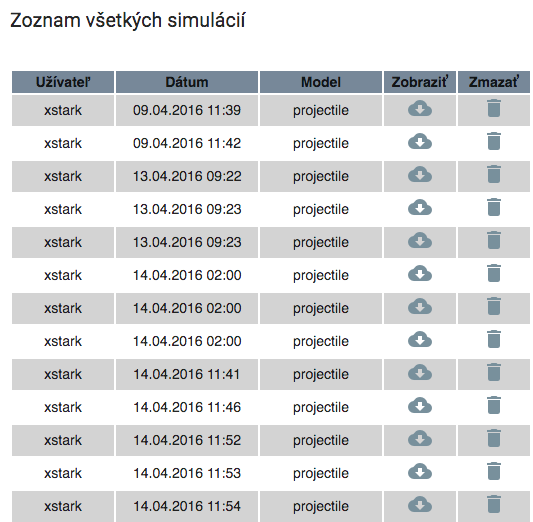
\includegraphics[scale=0.5]{img/code/angular-results-projectile.png}
  \caption{Zoznam uložených simulácií pre prihláseného užívateľa.}
  \label{img-angular-results-projectile}
\end{figure}

\begin{figure}[H]
  \centering
  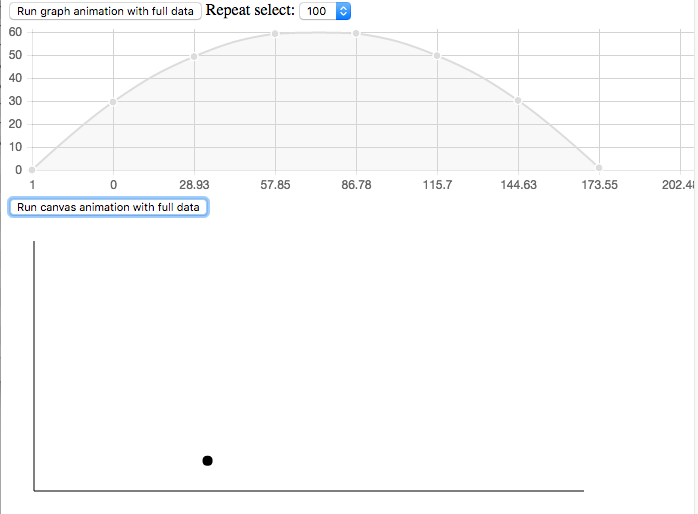
\includegraphics[scale=0.5]{img/code/angular-fulldata.png}
  \caption{Graf a animácia pre vybranú vzorku dát.}
  \label{img-angular-fulldata}
\end{figure}

Na webovej stránke sa ešte nachádza pod animáciou sa nachádza rovnaká tabuľka ako v obrázku č. \ref{img-angular-table} s rozdielom, že v tejto tabuľke sú kompletné údaje.


%\section{Inštalácia vytvoreného riešenia}
%asi lepsie do prilohy